\section{Approach}

\subsection{Overview}

To test the DFR tools, we first designed hypothetical test scenarios to simulate the challenges of real-world file recovery.
We then created each scenario in real file systems and saved them as raw images. 
Using the images as input, we ran each DFR tool and attempted to recover all deleted files. 
Finally, we compared the recovered files to their original versions in order to judge the tools' 
compliance with the NIST standards). A high-level view of the methodology for a typical test case is illustrated in Figure \ref{fig:overview}.

\begin{figure}[h]
    \centering
    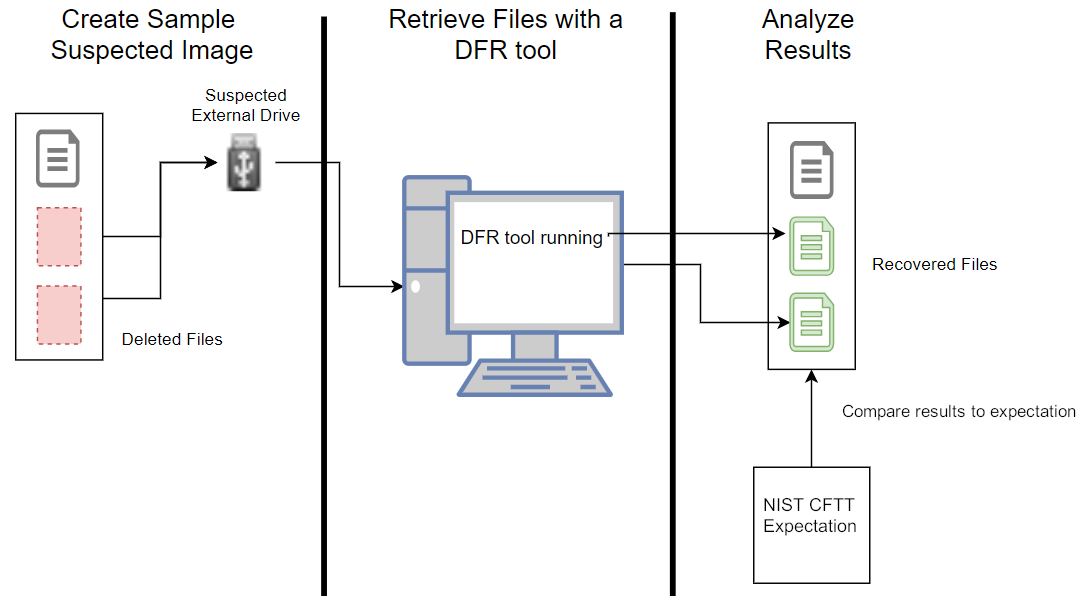
\includegraphics[width=\linewidth]{fig/overview.png}
    \caption{A filesystem containing deleted files is created on the external drive. That filesystem is then given as input to a DFR tool, which attempts to recover the deleted files. The recovered files are then analyzed to judge the DFR tool's compliance with the NIST CFTT standard.}
    \label{fig:overview}
\end{figure}

\subsection{Designing Recovery Scenarios}
To test the DFR tools' compliance with the standards, we designed a variety of scenarios in which a tool might have to recover a deleted file. 
We started with the simplest possible case: a file system containing just one deleted file. 
This case is ideal and trivial, but by adding more files, we can create a greater variety of scenarios.

The NIST standards limit their scope to recovery of files which were ``created and deleted in a process similar to how an end-user would create and delete files,''\cite{meta:dfr:standards} and exclude ``files and file system metadata that is specifically corrupted, modified, or otherwise manipulated to appear deleted.''\cite{meta:dfr:standards}
In other words, these standards address situations in which files were deleted via normal file system operations as implemented by a typical operating system, as opposed to direct modification of the file system by a user.
Within these constraints, there are two factors which can significantly complicate the file recovery process: 
fragmentation, and overwriting. 

These factors are thus the foundation of our test scenarios, with all cases besides the first involving either fragmented files, overwritten files, or a combination of both. 
The goal is to create test cases which are canonical; in other words, they constitute the basic elements of a file recovery scenario.
We suggest such a canonical list of test cases should be considered representative of all possible scenarios within the scope of the standards.

We designed the following test cases:
\begin{itemize}
    \item [1] Single deleted file
    \item [2] Fragmented deleted file, with an active file in between the fragments (Illustrated in Figure \ref{fig:case_2})
    \begin{figure}[h]
        \centering
        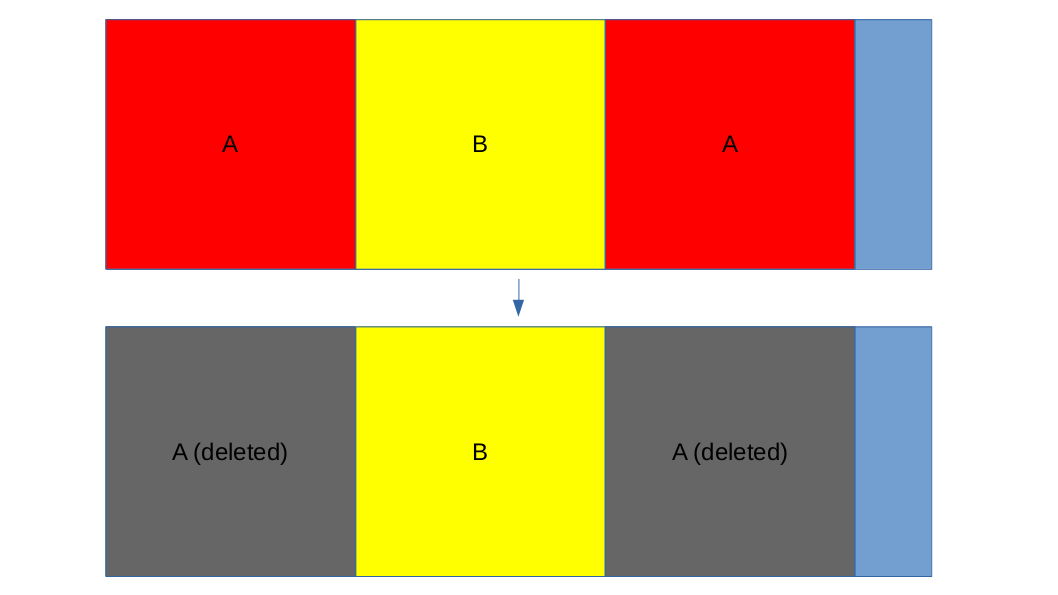
\includegraphics[width=\linewidth]{fig/case2.png}
        \caption{Test Case 2. Fragmented file A is deleted.}
        \label{fig:case_2}
    \end{figure}
    \item [3] Fragmented deleted file, with a deleted file in between the fragments
    \item [4i] Beginning of deleted file overwritten by an active file
    \begin{figure}[h]
        \centering
        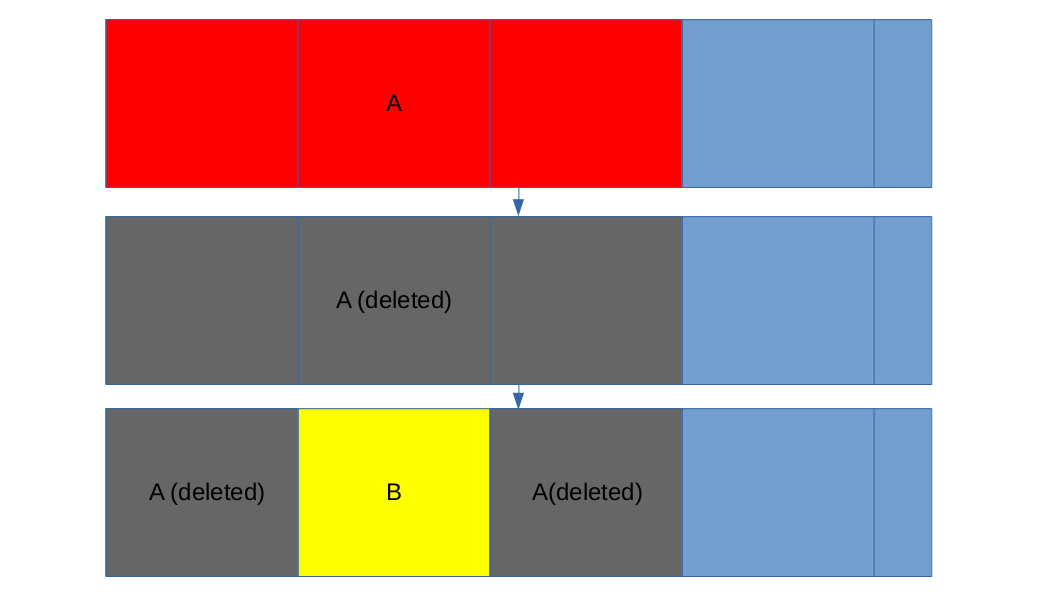
\includegraphics[width=\linewidth]{fig/case4ii.png}
        \caption{Test Case 4ii. Deleted file A is partially overwritten by file B.}
        \label{fig:case_4ii}
    \end{figure}
    \item [4ii] Middle of deleted file overwritten by an active file (Illustrated in Figure \ref{fig:case_4ii})
    \item [4iii] Deleted file partially overwritten by an active file which doesn't end on a sector boundary
    \item [4iv] Deleted file entirely overwritten by an active file
    \item [5i] Beginning of deleted file overwritten by another deleted file (Illustrated in Figure \ref{fig:case_5i})
    \item [5ii] Middle of deleted file overwritten by another deleted file
    \item [5iii] Deleted file partially overwritten by a deleted file which doesn't end on a sector boundary
    \item [5iv] Deleted file entirely overwritten by a deleted file
    \item [6] Fragmented deleted file, with an active file in between the fragments, with the second fragment overwritten by another active file (Illustrated in Figure \ref{fig:case_6})
    \begin{figure}[h]
        \centering
        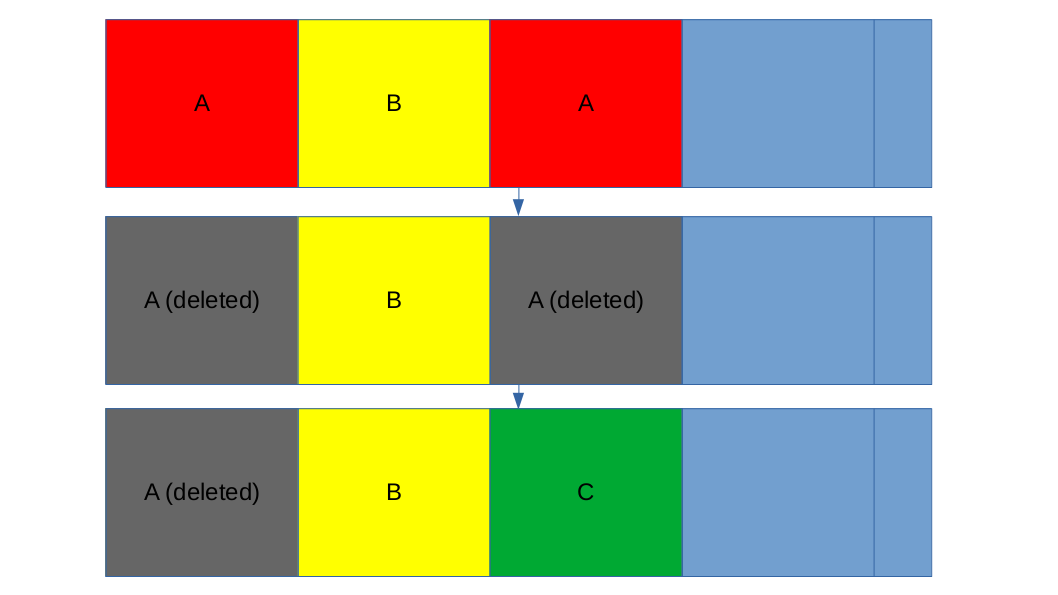
\includegraphics[width=\linewidth]{fig/case6.png}
        \caption{Test Case 6. Fragmented file A is deleted. File A is then partially overwritten by file C.}
        \label{fig:case_6}
    \end{figure}
    \item [7] Fragmented deleted file, with an active file in between the fragments, with the second fragment overwritten by another deleted file
    \begin{figure}[h]
        \centering
        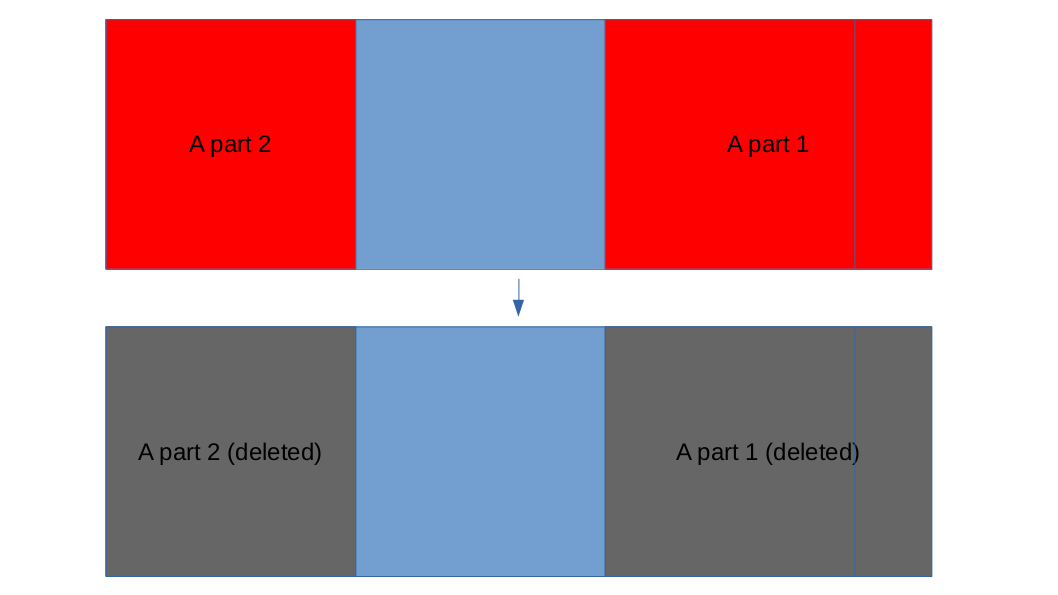
\includegraphics[width=\linewidth]{fig/case8.png}
        \caption{Test Case 8. Fragmented file A, which starts at the end of the filesystem and wraps around to the beginning, is deleted.}
        \label{fig:case_8}
    \end{figure}
    \item [8] Deleted file fragmented from the end of the file system to the beginning (Illustrated in Figure \ref{fig:case_8})
    \item [9] Deleted file fragmented from the end of the file system to after an active file
    \item [10] Deleted file fragmented from the end of the file system to after a deleted file

\end{itemize}

Because NTFS keeps track of the locations of all parts of a file even after deletion, fragmentation is not particularly interesting. Cases 8, 9, and 10 would be redundant with case 2, so we have excluded them for NTFS. Due to how NTFS allocates space for files, cases 4ii and 5ii cannot occur as a result of normal file operations, so they have also been excluded. No cases are excluded for FAT tests.

\subsection{Creating Test Images}
% Step by step process
All test file systems were created in partitions on a 32 GB flash drive. For each test case, the first step is to entirely write over the partition with zeros. This ensures all cases start from identical, reproduceable conditions. A new file system is written to the partition, then new files are written to the file system and deleted. The files used are simple text files containing one letter repeated (e.g. ``aa1M'' is 1 MiB of the letter 'a'). Files are written to the test file system by simply copying them from another drive. In some cases we also append data to a file in the test file system. Once the test file system matches the intended scenario, a read-only image of the partition is created. All tests are performed on these images rather than the original drive.

\subsubsection{Challenges}
% Caching problem
It is important to consider when creating test images that the low-level behavior of file operations is not always obvious. For example, when writing a file, there is no guarantee the file's data will be immediately written to the disk. The operating system may cache the operation and wait until the optimal time to perform the write, in order to maximize system performance. We observed this early on, as writing a file and subsequently deleting it would always result in the file's metadata being written, but often left no evidence of the file's data having ever existed. This behavior is obviously undesireable because it leaves nothing meaningful to be recovered. We resolved this by using the ``sync'' system call, which causes any such cached data to be immediately written to the disk, in between file writes and deletions. Unmounting the file system after writes has a similar effect.

% Learning and using the allocation algorithms
Another type of low-level behavior relevant to the image creation process is the allocation algorithm. The operating system must have some kind of algorithm to decide where in the data area new files should be written. Common allocation algorithms include ``first available,'' ``next available,'' and ``best fit.''
Learning and understanding whatever algorithm the OS uses is very helpful for forcing a specific arrangement of files. We observed that when writing to a FAT file system, Linux uses a ``next available'' algorithm. After the file system is mounted, the first write will start at the first free space in the data area. The next file will be written starting from the first free space after the previous file.
Meanwhile, when writing to an NTFS file system, Windows 10 appears to use a ``best fit'' algorithm. In this case, Windows tries to find the smallest space in which the file can fit without being fragmented, and write it there.

% Directory entries problem

\subsection{Recovering Files}

The settings we used when testing each tool are as follows:
For Autopsy\cite{autopsy}, we performed a standard recovery with all ingest modules disabled.
For Recuva\cite{recuva} we perfomed a standard recovery using the free version with default settings.
For FTK Imager\cite{ftk}, we performed a standard recovery using the free version with default settings.
For TestDisk\cite{testdisk} we used the ``file undelete'' feature under ``Advanced Filesystem Utils.''
For Magnet AXIOM\cite{axiom} we performed a ``full scan'' in AXIOM Process and exported all files accessible in ``Filesystem View'' in AXIOM Examine.

\subsection{Results}

After testing each tool, we analyzed the recovered object(s) from each test case. 
If the recovered file is identical to the original, obviously all standards have been met. 
While this is ideal, it is often impossible to perfectly recover a file (such as when it is overwritten) so the standards do not require it. 
In our results, the file is only ever recovered perfectly in FAT cases 1 and 2, and NTFS cases 1-3. 
For all other cases, the tool is judged on each core feature individually. 
These judgements are summarized in Figure \ref{fig:results_fat} for FAT test cases and Figure \ref{fig:results_ntfs} for NTFS test cases.

\begin{figure*}[h!]
    \centering

    \begin{subfigure}{0.17\linewidth}
        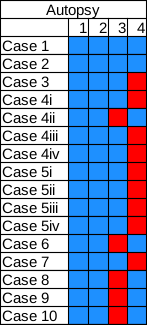
\includegraphics[width=\linewidth]{fig/autopsy_results_fat.png}
        \subcaption{Autopsy}
    \end{subfigure}~~
    \begin{subfigure}{0.17\linewidth}
        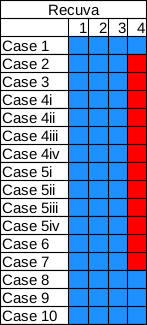
\includegraphics[width=\linewidth]{fig/recuva_results_fat.png}
        \subcaption{Recuva}
    \end{subfigure}~~
    \begin{subfigure}{0.17\linewidth}
        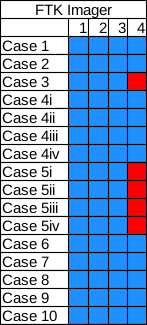
\includegraphics[width=\linewidth]{fig/ftk_results_fat.png}
        \subcaption{FTK}
    \end{subfigure}~~
    \begin{subfigure}{0.17\linewidth}
        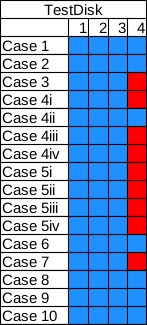
\includegraphics[width=\linewidth]{fig/testdisk_results_fat.png}
        \subcaption{TestDisk}
    \end{subfigure}~~
    \begin{subfigure}{0.17\linewidth}
        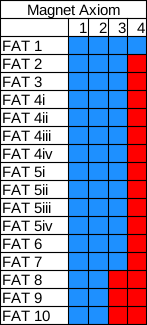
\includegraphics[width=\linewidth]{fig/axiom_results_fat.png}
        \subcaption{Magnet AXIOM}
    \end{subfigure}~~
        
    \caption{Test results on FAT test cases for each DFR tool. Rows represent test cases whereas columns represent NIST core features. Blue is passing, red is failing, grey is not tested.}
    \label{fig:results_fat}
\end{figure*}

\begin{figure*}[h]
    \centering

    \begin{subfigure}{0.17\linewidth}
        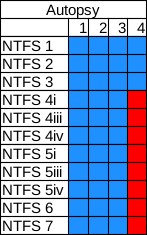
\includegraphics[width=\linewidth]{fig/autopsy_results_ntfs.png}
        \subcaption{Autopsy}
    \end{subfigure}~~
    \begin{subfigure}{0.17\linewidth}
        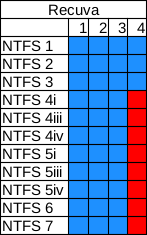
\includegraphics[width=\linewidth]{fig/recuva_results_ntfs.png}
        \subcaption{Recuva}
    \end{subfigure}~~
    \begin{subfigure}{0.17\linewidth}
        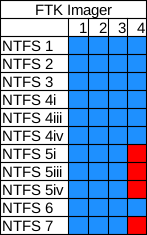
\includegraphics[width=\linewidth]{fig/ftk_results_ntfs.png}
        \subcaption{FTK}
    \end{subfigure}~~
    \begin{subfigure}{0.17\linewidth}
        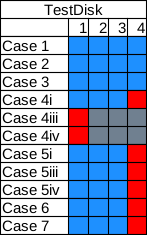
\includegraphics[width=\linewidth]{fig/testdisk_results_ntfs.png}
        \subcaption{TestDisk}
    \end{subfigure}~~
    \begin{subfigure}{0.17\linewidth}
        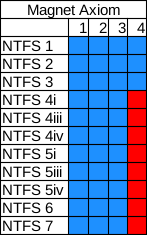
\includegraphics[width=\linewidth]{fig/axiom_results_ntfs.png}
        \subcaption{Magnet AXIOM}
    \end{subfigure}~~
        
    \caption{Test results on NTFS test cases for each DFR tool. Rows represent test cases whereas columns represent NIST core features. Blue is passing, red is failing, grey is not tested.}
    \label{fig:results_ntfs}
\end{figure*}

For cases in which a tool does not fulfull core feature 1, in other words, it cannot find a deleted file, we make no judgement about the remaining core features.

\subsubsection{Recovering Fragmented Files}
In cases of fragmentation in FAT file systems, we found each tool generally approaches recovery in one of two ways. 
Recuva and Magnet AXIOM start from the beginning of the file and recover the full length of the file even if an active file exists in that space. 
Autopsy, FTK, and TestDisk will start from the beginning of the file and recover the full length, but skip over any active files they encounter.
Autopsy, FTK, and TestDisk recover all of file A, while Recuva and Magnet AXIOM's recovered images erroneously contain data from file B, causing them to fail core feature 4. 
When the space in between fragments is unallocated, all tools recover the file as though it was contiguous, pulling some erroneous data and failing core feature 4. 
When the fragmentation occurs at the end of the file system, Recuva, FTK, and TestDisk recover only the first fragment, while Autopsy returns a short file of null data, and Magnet AXIOM reports an error and returns an empty file.
Cases with fragmentation are trivial for NTFS file systems as more information is available from the metadata. 
Unsurprisingly, no tools had problems with fragmentation cases for NTFS.

\subsubsection{Recovering Overwritten Files}
In cases where a file has been overwritten by an active file, we found most tools recover the deleted file as though it is not overwritten, failing core feature 4. 
A few exceptions are FTK Imager, which recovers the file up to the point where it has been overwritten, and Autopsy, which generally recovers only the first cluster of an overwritten file in FAT, and behaves like the other tools for NTFS. 
TestDisk also exhibits the same behavior as FTK for FAT case 4ii only. 
Strangely, Magnet AXIOM's recovered objects for FAT cases 4i and 4ii include the overwritten sections, but nothing after them.
Other Magnet AXIOM results were similar to the other tools.
When the overwriting file has also been deleted, all tools recover the first file as though it is not overwritten.

\subsubsection{Abnormal Results}
A few results stand out as unusual.
These are cases for which it is difficult to infer from the recovered object what approach a tool is using.

For FAT cases 4ii, 6, 8, 9, and 10, Autopsy returns a 1.5 KiB file of null data.
1.5 KiB is equivalent to 3 sectors, while a FAT cluster in our cases is defined as 4 sectors (2 KiB).

TestDisk fails to identify a file for NTFS cases 4iii and 4iv only. 
These are the only test cases in which a tool does not fulfill core feature 1.

For FAT cases 4i and 4ii, Magnet AXIOM does not recover the entire length of the deleted file, but it also does not exclude the overwritten sections. 
In both cases, it recovers up to the end of the overwritten sections, rather than up to the beginning like FTK does.
